\section{Дрейф, вызванный искривлением магнитных силовых линий} 

Для расчета скорости этого дрейфа введем локальную систему отсчета, вращающуюся вокруг центра кривизны $С$ магнитной силовой линии (см. рис. \ref{202}).

\begin{figure}[h!]
    \centering
    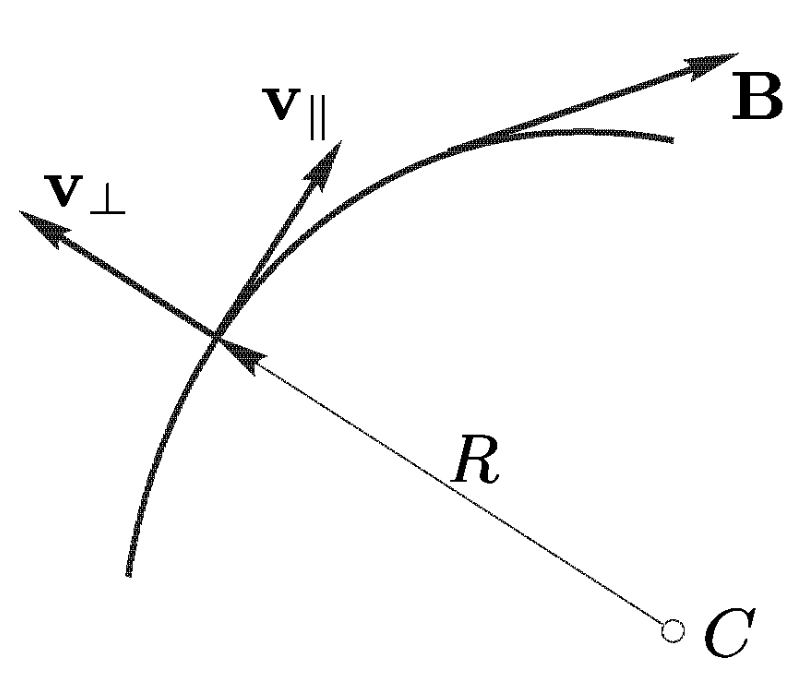
\includegraphics[scale=0.2]{202.png}
    \caption{}
    \label{202}
\end{figure}

Ось вращения направим параллельно бинормали $\mathbf{b}$ этой силовой линии (она перпендикулярна к плоскости рисунка). Числовое значение угловой скорости вращения $\Omega$ определим из условия $\mathbf{v_{\Vert}} = [\mathbf{\Omega R}]$. Тогда в рассматриваемой локальной системе отсчета частица будет иметь только поперечную скорость $v_{\perp}$, которая играет роль относительной скорости $v_{отн}$ При рассмотрении движения в локальной системе отсчета к действующим силам надо добавить две силы инерции: кориолисову и центробежную. Силу инерции, вызванную неравномерностью вращения, учитывать не надо, так как она может влиять на дрейф частицы лишь во втором или высшем порядке малости. Кориолисова сила инерции $2m [\mathbf{v_{отн} \Omega}] = 2m \Omega [\mathbf{v_{\perp} b}]$ направлена вдоль силовой линии, а потому она будет изменять только продольную составляющую $v_{\Vert}$ скорости $\mathbf{v}$. Центробежная сила инерции $m v_{\Vert}^2 \mathbf{R} / R^2$ вызовет дрейф в перпендикулярном направлении. Скорость этого дрейфа определяется выражением:

\[
    v_д = \frac{c}{B^2 e} \left[ \frac{m v_{\Vert}^2}{R^2} \mathbf{R B} \right] = - \frac{m c v_{\Vert}^2}{B e R} [\mathbf{N h}]
\]

Если $\mathbf{N}$ — единичный вектор главной нормали к магнитной силовой линии, то $\mathbf{R} = — R \mathbf{N}$. Поэтому, полагая в последнем соотношении $\mathbf{B} = B \mathbf{h}$. и учитывая, что $\mathbf{b} = [\mathbf{hN}]$, получим

\begin{equation}
    v_д = \frac{m c v_{\Vert}^2}{B R e} \mathbf{b}
\end{equation}

Поскольку дрейф, выражаемый этой формулой, вызывается центробежной силой инерции, он называется \textit{центробежным дрейфом}.
